\documentclass[ex]{exercise}

\deadline{05.12.2023}

\begin{document}

\section{Quarz-Plättchen}
Die Hauptbrechungsindizies für Quarz sind \(n_{o}=1.5443\) und \(n_{ao}=1.5534\). Wie dick muss ein 
Quarz-Plättchen sein, damit es für Licht der Wellenlänge \(550 \u{nm}\) als \(\lambda/4\)-Plättchen wirkt?

\dottedlinete

\begin{align*}
    \Delta s_{\te{optisch}} &= d \Delta n\\
    \frac{\lambda}{4} &= d \Delta n\\
    d &= \frac{\lambda}{4\Delta n}\\
    &= \frac{550\u{nm}}{4\cdot (1.5534 - 1.5443)}\\
    &= 15.1 \u{\mu m}
\end{align*}

\section{Polarisationsfilter Reihenschaltung}
Sie schicken linear polarisiertes Licht durch drei hintereinander stehenden linear Polarisationsfiltern.
Die Ausrichtung der Filter sind \(30^\circ\) zum vorherigen Filter gedreht, wobei der Erste 
gleicherma{\ss}en zur Polarisationsrichtung des einfallenden Lichts gedreht ist. Was 
ergibt sich für die Intensiät des Lichs nachdem dritten Filter?

\dottedlinett

Nach dem Gesetz von Malus gilt:
\begin{align*} 
    I' &= I \cdot \cos^2\Delta\theta\\
    I'_{\te{rel}} &= \cos^2\Delta\theta\\
    I'_{\te{rel},3\te{-Filter}} &= \hug{\cos^2\Delta\theta}^3=\cos^6\Delta\theta\\
    &= \cos^6 \frac{30\cdot 2\pi}{360}\\
    &\approx 0.422 
\end{align*}

\section{Brewster-Winkel}
Berechnen Sie den Polarisationsgrad \(P\) des reflektierten Lichtes, das mit dem Winkel
\(\alpha=45^\circ\) auf einer Glasplatte mit der Brechzahl \(n=1.52\) einfällt.

\subsection{}
Zeigen Sie dazu zunächst, dass für die Intensitäten der zur Einfallsebene parallel \(p\)
und normalen \(n\) Anteile des reflektierten Lichts gilt
\begin{align*}
    I_p^r = \frac{I_0}{2} \hug{\frac{\tan(\alpha-\beta)}{\tan(\alpha+\beta)}}^2
    \qquad I_n^r = \frac{I_0}{2} \hug{\frac{\sin(\alpha-\beta)}{\sin(\alpha+\beta)}}^2
\end{align*}
Mit dem Brechwinkel im Glas \(\beta\) und \(I_0\) der gesamt Intensität des einfallenden 
unpolarisierten Lichts.

\dottedlinett

Ausgehend von den Fresnel'schen-Formeln gilt:
\begin{align*}
    r_n &= \frac{n_1\cos\alpha - n_2\cos\beta}{n_1\cos\alpha + n_2\cos\beta}\\
    r_p &= \frac{n_2\cos\alpha - n_1\cos\beta}{n_2\cos\alpha + n_1\cos\beta}
\end{align*}
Und damit:
\begin{align*}
    I_n^r &= \frac{E_n^2}{2} \\
    &= \frac{E_0^2 r_n^2}{2} \\
    &= \frac{I_0^2}{2} \hug{\frac{n_1\cos\alpha - n_2\cos\beta}{n_1\cos\alpha + n_2\cos\beta}}^2\\
    &= \frac{I_0^2}{2} \hug{\frac{n_1\cos\alpha - n_1 \frac{\sin \alpha}{\sin\beta}
    \cos\beta}{n_1\cos\alpha + n_1 \frac{\sin \alpha}{\sin\beta}\cos\beta}}^2\\
    &= \frac{I_0^2}{2} \hug{\frac{\cos\alpha\sin\beta - \sin\alpha\cos\beta}
    {\cos\alpha\sin\beta + \sin\alpha\cos\beta}}^2\\
    &= \frac{I_0^2}{2} \hug{\frac{\sin(\alpha-\beta)}{\sin(\alpha+\beta)}}^2\\
\end{align*}
\begin{align*}
    I_p^r &= \frac{E_p^2}{2} \\
    &= \frac{E_0^2 r_p^2}{2} \\
    &= \frac{I_0^2}{2} \hug{\frac{n_2\cos\alpha - n_1\cos\beta}{n_2\cos\alpha + n_1\cos\beta}}^2\\
    &= \frac{I_0^2}{2} \hug{\frac{n_1 \frac{\sin \alpha}{\sin\beta}\cos\alpha - n_1\cos\beta}{n_1 \frac{\sin \alpha}{\sin\beta}\cos\alpha + n_1\cos\beta}}^2\\
    &= \frac{I_0^2}{2} \hug{\frac{\sin \alpha\cos\alpha - \sin\beta \cos\beta}
    {\sin \alpha\cos\alpha +\sin\beta \cos\beta}}^2\\
    &= \frac{I_0^2}{2} \hug{\frac{\tan(\alpha-\beta)}{\tan(\alpha+\beta)}}^2\\
\end{align*}



\subsection{Berechnen Sie \(P\).}
\begin{align*}
    I_p^r  &\approx 0.00423\\
    I_n^r  &\approx 0.0460\\
    P &= \frac{I_{\te{pol}}}{I_{\te{ges}}}= \frac{\max\hug{I_p^r,I_n^r}}{I_p^r+I_n^r}= \frac{I_n^r}{I_p^r + I_n^r}\\
    &\approx 0.916
\end{align*}

\subsection{Berechnen Sie den Winkel \(\delta\) bei der das reflektierte Licht vollständig polarisiert.}
\begin{align*}
    0 &\peq I_p^r\\
    \implies 0&= r_p\\
    &= \frac{n_2\cos\alpha - n_1\cos\beta}{n_2\cos\alpha + n_1\cos\beta}\\
    &= n_2\cos\alpha - n_1\cos\beta\\
    &= n_2\cos\alpha - n_1\cos\hug{\arcsin\hug{\frac{n_1}{n_2}\sin\alpha}}\\
    &= n_2\cos\alpha - n_1\sqrt{1- \frac{n_1^2}{n_2^2}\sin^2\alpha}\\
    &= n_2^2\cos^2\alpha - n_1^2\hug{1- \frac{n_1^2}{n_2^2}\sin^2\alpha}\\
    &= \frac{n_2^2}{n_1^2}\cos^2\alpha + \frac{n_1^2}{n_2^2}\sin^2\alpha - 1\\
    &= \frac{n_2^2}{n_1^2}\frac{1}{1+ \tan^2\alpha} + \frac{n_1^2}{n_2^2}\frac{\tan^2\alpha}{1+ \tan^2\alpha} - 1\\
    &= \frac{n_2^2}{n_1^2} + \frac{n_1^2}{n_2^2}\tan^2\alpha - 1 - \tan^2\alpha\\
    &= \frac{n_2^2}{n_1^2} + \hug{\frac{n_1^2}{n_2^2}-1}\tan^2\alpha - 1\\
    \alpha &= \arctan\sqrt{\frac{1 - \frac{n_2^2}{n_1^2}}{\frac{n_1^2}{n_2^2} - 1}}\\
    &= \arctan\sqrt{\frac{\frac{n_2^2}{n_1^2}\hug{1 - \frac{n_2^2}{n_1^2}}}{1 - \frac{n_2^2}{n_1^2}}}\\
    &=\arctan \frac{n_2}{n_1}\\
    &\approx 0.983 \approx 56.3 ^\circ
\end{align*}

\section{Wollaston-Prisma}
Zwei Prismen aus Kalkspat, die so geschnitten sind, dass die optische Achse einmal in der
Zeichenebene, zum anderen senkrecht zur Zeichenebene verläuft, werden zusammengeklebt,
wobei die optische Wirkung des Klebers selbst vernachhlässigt werden kann. 
Die Hauptbrechungsindeizes für Kalkspat sind \(n_0=1.6584\) und \(n_{ao}=1.4864\).
Ein unpolarisierter Lichtstrahl, der senktrecht zur optischen Achse der ersten Prismas einfällt, 
spaltet beim Durchgang durch diese optische System in zwei gebrochene Lichtstrahlen 
\(S1\) und \(S2\) auf (siehe Skizze).

\subsection{Wie sind die beiden Lichtstrahlen polarisiert?}
Die beiden Lichtstrahlen sind zu \(100\%\) polarisiert, wobei \(S1\) in der Ebene schwingt 
(ordentlich im ersten Keil)
und die Schwingung von \(S2\) aus der Ebene raus kommt (au{\ss}erordentlich im ersten Keil).

\subsection{Wie gro{\ss} ist der Winkel zwischen den beiden Strahlen \(S1\) und \(S2\),
wenn der Keilwinkel \(\gamma=15^\circ\)?}

\dottedlinett

Der Anteil des Lichtstrahls, der im ersten Keil ordentlich ist, d.h. 
aus der Ebene schwingt, wird im Übergang zum zweiten Keil au{\ss}erordentlich, es 
gilt daher nach dem Snell'schen Gesetz:
\begin{align*}
    n_o \sin\alpha_o &= n_{ao} \sin\beta_o\\
\end{align*}
Und analog für den Teil des Strahls, der im ersten Keil au{\ss}erordentlich ist:
\begin{align*}
    n_{ao} \sin\alpha_{ao} &= n_{o} \sin\beta_{ao}\\
\end{align*}
Aus der Geometrie folgt au{\ss}erdem:
\begin{align*}
    \alpha_{o}&= 
    \alpha_{ao} = \gamma 
\end{align*}
Damit gilt:
\begin{align*}
    \beta_{o} &= \arcsin\hug{\frac{n_o}{n_{ao}} \sin\gamma}\approx 0.293\\
    \beta_{ao} &= \arcsin\hug{\frac{n_{ao}}{n_o} \sin\gamma}\approx 0.234\\
\end{align*}

Beim Austritt aus dem zweiten Keil, werden die beiden Lichtstrahlen erneut gebrochen, 
es gilt aufgrund der Geometrie:
\begin{align*}
    \alpha' &= \beta - \gamma 
\end{align*}
und somit:
\begin{align*}
    \beta'_o &= \arcsin\hug{n_{ao}\sin(\beta_o - \gamma)} \approx 0.0463 \\
    \beta'_{ao} &= \arcsin\hug{n_{o}\sin(\beta_{ao}- \gamma)} \approx -0.0459
\end{align*}
Damit ist \(\alpha = \beta'_{o} - \beta'_{ao}\approx 0.0922\approx 5.28^\circ\). 

\section{3D-Brillen}
\subsection{}
Dass man der Filter vor dem offenen Auge im Spiegel schwarz erscheint, 
lässt sich wie folgt erklären:
\begin{enumerate}
    \item Das vom Auge reflektierte Licht ist zunächst unpolarisiert, und 
    wird auf dem Weg durch die 3D-Brille zirkular polarisiert. Dafür muss die Brille 
    entweder aus einem linearen Polfilter bestehen, hinter dem ein \(\lambda/4\)-Plättchen geklebt ist,
    oder aus einem chiralem Molekül hergestellt worden sein.
    \item Trifft das Licht auf den Spiegel, wird es nicht nur reflektiert, es 
    wechselt sich auch die Richtung der Polarisation, wie an der folgenden Skizze 
    nachvollzogen werden kann:
    \begin{figure}[H]
        \centering
        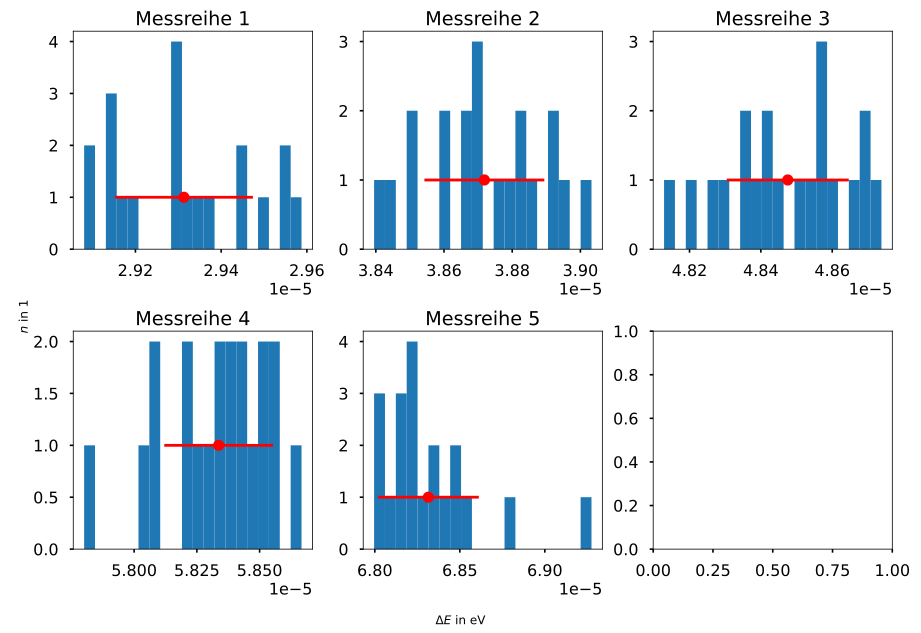
\includegraphics[width=0.7\textwidth]{1.jpg}
        \caption{Skizze der Reflektion eines zirkular polarisierten Lichtstrahls}
    \end{figure}
    Man sieht auf der Skizze einen zirkular polarisierten Lichtstrahl, als Superposition 
    zweier entgegengesetzter linear polarisierter Lichtstrahlen (rot/grün). Der Strahl ist
    zu diesem Zeitpunkt linkdrehend. Wird der Strahl nun an der eingezeichneten Ebene 
    reflektiert, erfährt die rote Welle einen \(180^\circ\) Phasensprung (die rückkehrende 
    Welle ist grün eingezeichnet); Die blaue Welle hingegeben behält ihre Phase bei. 
    Schaut man sich die zurückkehrende Welle in der Gesamtheit an, 
    fällt auf, dass sie nun rechtsdrehend ist, die Polarisation hat sich also gewechselt.

    \item Das zurückkehrende Licht kann nun nicht mehr durch das Brillenglas des offenen
    Auges, da die Polarisation genau entgegengesetzt ist. Das Glas des offenen Auge 
    erscheint daher schwarz.
\end{enumerate}
Dass das Brillenglas des geschlossenen Auges weiterhin durchsichtig ist, liegt daran,
dass der Filter auf diesem Auge entgegengesetzt polarisiert ist. Nach dem gleichem Schema
wie oben ergibt sich daher, dass der zurückkehrende Strahl die gleiche Polarisation wie der Filter 
des offenen Auges hat, man kann daher durch den Filter durchschauen.

\subsection{}
Dreht man die Brille um, würde das Licht von hinter den Brillengläsern erst das \(\lambda/4\)-Plättchen 
passieren, und dann den linearen Polfilter. Das Licht, dass am Spiegel reflektiert wird ist somit
in diesem Fall nicht zirkular, sondern linear polarisiert, und wechselt daher am Spiegel die Polarisation nicht.
Das Licht des offenen Auges, kann daher ohne Probleme wieder den Filter passieren, 
anders als das Licht, welches vom geschlossenen Auge ausgeht, dieses wird nun vom Filter des offenen Auges absorbiert.
Nach meiner Erklärung würde das Umdrehen der Brille somit zur Folge haben, dass das sichtbare Auge sich 
wechselt. Realisiert man den zirkularen Filter hingegen mit einem chiralen Molekül, würde 
sich die Beobachtung durch drehen der Brille nicht ändern, da diese Art Filter symmetrisch ist, d.h. es wäre 
immer das ungeöffnete Auge zu sehen. 

\end{document}